\chapter{Methods}
\label{chapter4}
We propose a framework that synthesises planning and reinforcement learning which can overcome the inherent inaccuracies of models whilst constraining exploration  and improving sample efficiency by hypothesising, through reasoning, changes to the model that would be most beneficial to the planner and then planning on this temporary model to guide exploration. The correctness of these changes is then realised through experience in the real environment, and the model is updated.
We use the principle of \textit{optimism in the face of uncertainty}, we state that we are always almost in a state of uncertainty due to the inevitable inaccuracies of the model.
To enable the planner to make these hypotheses we equip it with additional actions which we denote Meta Actions.

\section{The Framework}
We assume that the environment has a discrete state space, $S$, or a state space that can be discretised, a finite action space, $A$, with deterministic or stochastic dynamics which can be described by a transition function, $T$, and deterministic rewards which can be described by a reward function, $R$. Therefore, we assume that the environment can be modelled as an MDP $E = (S, A, T, R)$. The goal of the framework is to produce a policy $\pi_E$ which maximises the cumulative reward received when acting in the environment $E$.
Additionally, we assume that an attempt at modelling the environment has been made and embedded in an MDP $M = (S, A, T', R')$, where the same conditions hold for $T'$ and $R'$ as for $T$ and $R$. We do not expect or require $M$ to be accurate. We learn a $Q$-Function, $Q$, which a policy can be derived from. The choice of initialisation open.
\\Our framework consists of two phases, a planning phase and a model-free phase. Since we only consider episodic tasks, the agent is given a finite number of episodes, $N_p$, for the planning phase, thereafter until termination (some finite number of episodes has been completed), the model-free phase takes over.

%  Since we only consider episodic tasks, the agent is given a finite number of episodes, $N_p$ for the planning phase. The planning phase performs exploration and computes initial estimates for the Q-Values, $Q$. The model-free phase bootstraps from the initial Q-Value estimates and carries out model-free learning, following the policy $\pi_Q$, refining the estimate and continually updating the Q-Values.
\section{The Planning Phase}
The planning phase has three distinct steps: planning (and hypothesising), execution and learning, which can be seen in Figure \ref{fig:framework}. Throughout the planing phase we maintain a tabular likelihood model, therefore we maintain a table $n$ which maps state-action-state triples to integers; for instance $(0, 1, 0) \rightarrow 3$ means that the transitions $(0, 1, 0)$ has been observed three times.
\subsection{Planning}
The Planner begins by constructing a temporary model, $M'$ which is initially a copy of $M$. The planner maintains a plan until model-learning occurs, when it replans.
\subsubsection{Meta Actions}
These actions do not cause the agent to act in the environment, and thus do not return any observation in terms of a new state and a reward, but rather cause changes directly to the model when called upon. An important factor and one of the main difficulties is deciding what Meta Actions should be exposed to the planner and when the planner should be able to invoke the Meta Actions. Therefore, we state three conditions which all must hold for a Meta Action to be invoked: a Meta Action must be admissible, feasible and reasonable.
\\A Meta Action is admissible if applying it to the model leads to what seems like a better plan. If applying the Meta Action does not result in any benefit to the planner, but rather it negatively affects the planner, then it should not be called. In-fact due to the nature of planning, an inadmissible Meta Action would never be called.\\Feasibility is important, since it ensures that we don't contradict observations and don't infinitely hypothesise changes to the model. However, the definition of feasibility depends on the transition dynamics of the domain. In the deterministic case, a Meta Action is feasible if the state or state-action pair that it affects has not been previously observed, and changes to to that state or state-action pair have not been previously hypothesised.
For stochastic domains, the latter condition of deterministic domains is sufficient for a Meta Action to be feasible.
\\Often, the change to the model that would be of most benefit the planner, is to simply add a transition from the current state to the goal state. However, this is almost never going to be a change that is realised to be correct; and instead would lead to behaviour akin to taking a random-walk through the state space until the goal is reached and the Meta Actions have been exhausted. Hence, it's key that an additional constraint exists, that ensures Meta Actions which are called hypothesise reasonable changes to the model. We consider two key ways of determining reasonability: through embedding reasonable Meta Actions in the model by-hand and through learning Meta Actions directly from experience.
\subsection{Execution}
At discrete time steps, $t$, the agent samples an action $a$ from the planner, and executes it. At time $t+1$ it observes its new state $s'$ and the scalar reward signal.
\subsection{Learning}
We begin by updating the observation table $n$ with the observed transition. Then, we update the model, $M$ (if necessary). Furthermore, the $Q$-Function is updated according to the new state and reward received.
\section{The Model-Free Phase}
The model-free phase has three distinct steps: action selection, execution and learning, which can be seen in Figure \ref{fig:framework}.
\subsection{Action Selection}
An action is selected greedily with respect to the $Q$-function.
\subsection{Execution}
\subsection{Learning}
The $Q$-Function is updated according to the new state and reward received.
% \subsection{Planning}
% The choice of planner is largely irrelevant to the framework, we mostly consider heuristic search algorithms, through A*, and planning by dynamic programming, through Value Iteration. Value Iteration was chosen over Policy Iteration as it tends to be more efficient, and since we are performing VI many times; this is very beneficial. However, it is important for the planner to be able to quantitatively evaluate plans; planning by VI was a good option here, since it computed a Value Function as an intermediate step, and we could use that for evaluation.
% A temporary model is created. The planner then begins planning on this model, at each node (state), the planner considers both the actions and available Meta Actions - if a Meta Action is chosen, then that change is made to the temporary model and planning continues. The computed plan is then returned to the agent.
% \subsection{Execution}
% During the planning phase, the agent chooses actions by sampling a plan from the planner. During the model-free phase, the agent chooses actions from the learned policy. The agent then executes the action in the environment, observing its affects through its new state and the reward received.
% \subsection{Learning}
% There are two sections to the learning step: where the model is learned \citeppp{10.1145/122344.122377}, and  where the policy is learned. The model is learned, as a tabular maximum likelihood model. The policy is learned, by at each discrete time step  updating the maintained Q-values using Q-Learning.
% We acknowledge the fact that tabular maximum likelihood approach and tabular Q-function approaches do not scale well to large, continuous, state spaces, however the environments that we were interested in within this work had finite, discrete state spaces (or they could be discretised) which were not too large to suffer from the \textit{curse of dimensionality}. Moreover, these two choices allowed for simplifications to be made for ease of implementation. Q-Learning was chosen over SARSA, as it allows the optimal policy to be learned without actually following the optimal policy; this is key to the planning phase, where due to the hypotheses made, the policy being followed may not be optimal.
\section{Implementations}
The description of the framework above led to various implementations. The underlying concept of allowing the planner to hypothesise changes to the model is present throughout all of the frameworks, but the ways in which the planner decides which change is most beneficial differs, and in some places simplifications are offered for differing domains (deterministic vs stochastic). Each framework will be presented and highlighted here.
\subsection{RL-A* Meta, embedded reasonable actions (Deterministic)}
This was an early implementation, specifically aimed at deterministic gridworlds; and it is only really suitable for them, as A* doesn't work well with stochasticity and heuristics are difficult to design for non-navigation based tasks. The cost function was simply the absolute value of the reward function, and the heuristic chosen was the Manhattan Distance \citep{krause1973taxicab}.
\\The Meta Actions that were available to the planner allowed it to add/remove obstacles, and increase/decrease rewards for state-action-state tuples, reasonable meta actions were embedded in the model by-hand.
\subsection{RL-A* Meta, embedded reasonable actions, with short-term memory (Stochastic)}
An extension of RL-A* Meta that attempts to deal with stochasticity. The A* implementation was modified, such that the cost function was the absolute value of the reward function multiplied by 1 minus the probability of achieving that reward.
\\To deal with the issue of stochasticity, and to encourage the agent to explore states again that it might have got unlucky with previously, the agent had a short-term memory; it only accounted for the previous $N$ episodes when contemplating, its observations and Meta Actions it had already called, during planning.
\subsection{RL-VI Meta, embedded reasonable actions}
To deal with varying domains, a different planner needed to be used. We opted for planning by dynamic programming, through Value Iteration, as the Value Function provided us with something to easily measure if a plan was "better".
\\The Meta Actions that were available to the planner allowed it to add/remove transitions, and increase/decrease rewards for state-action-state tuples, reasonable meta actions were embedded in the model by-hand.
\\Starting with an initial estimate of the Value Function (which is updated each time the model is updated through experience), during planning, at each state we hypothesise candidate changes to the model and compute a new Value Function for that state; if it's greater than the current, then the change is accepted.
\\This implementation worked for deterministic and stochastic domains, due to the nature of Value Iteration.
\subsection{RL-VI Meta, with learning reasonable Meta Actions}
The overall implementation is the same as RL-VI Meta, except Meta Actions are learned and obtained through experience, rather than embedded by-hand in the model. A Meta Action is learned when a discrepancy is noticed between the model and the real environment; this change that was applied to the model through model-learning becomes an action that can be invoked later on.


\begin{figure}[h!]
    \centering
    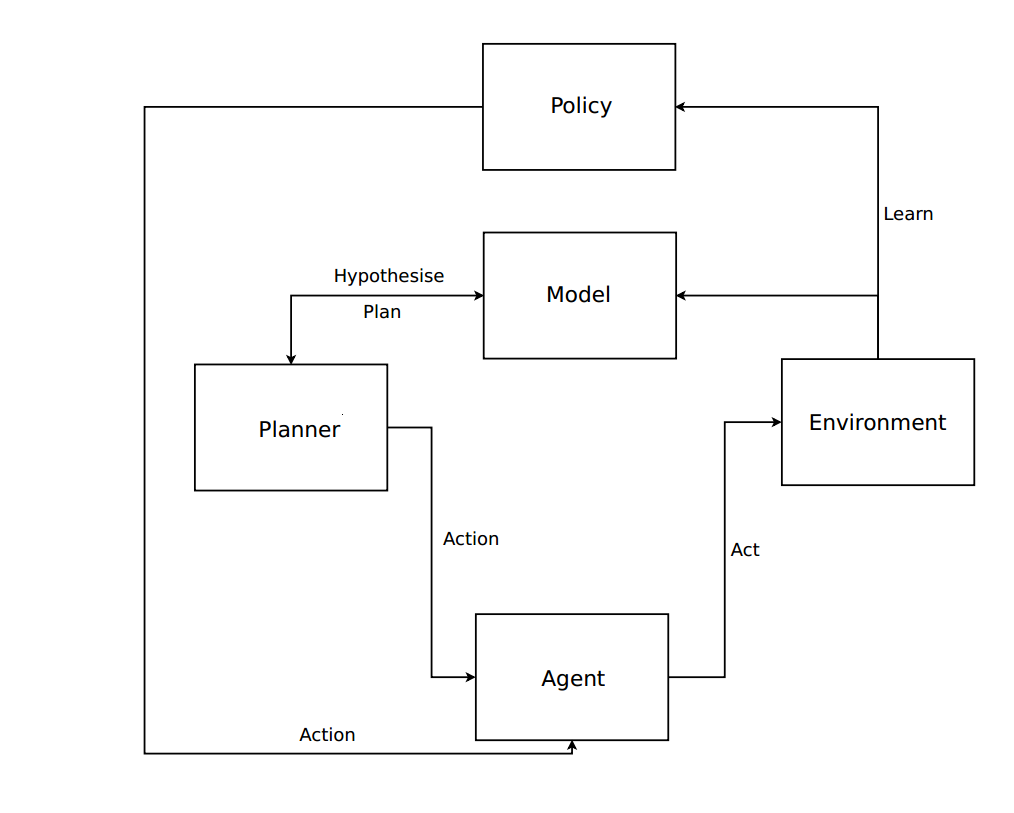
\includegraphics[max size={\textwidth}{\textheight}]{report/assets/diagram.png}
    \caption{Framework}
    \label{fig:framework}
\end{figure}
\section{Link to Human Decision Making}
\begin{itemize}
    \item What if that road is busy today, etc.?
\end{itemize}